% Panel 1 – Genome structure diagram.
%
% Compile standalone:
%   pdflatex panel1_genome.tex
%
% Include in paper:
%   % Panel 1 – Genome structure diagram.
%
% Compile standalone:
%   pdflatex panel1_genome.tex
%
% Include in paper:
%   % Panel 1 – Genome structure diagram.
%
% Compile standalone:
%   pdflatex panel1_genome.tex
%
% Include in paper:
%   % Panel 1 – Genome structure diagram.
%
% Compile standalone:
%   pdflatex panel1_genome.tex
%
% Include in paper:
%   \input{figures/panel1_genome.tex}   (inside a figure environment)
%
% Layout:
%   δ (seam positions, continuous)  |  ρ (grain rotation)  |  κ (tex. phase)  |  π (nesting order)  |  h
%   2M floats in [0,1]              |  S ints in {0..3}    |  S ints in {0..K-1}  |  S-permutation  |  int

\documentclass[tikz, border=6pt]{standalone}
\usepackage{tikz}
\usetikzlibrary{decorations.pathreplacing, calc, positioning}
\usepackage{amsmath}
\usepackage{amssymb}

\begin{document}
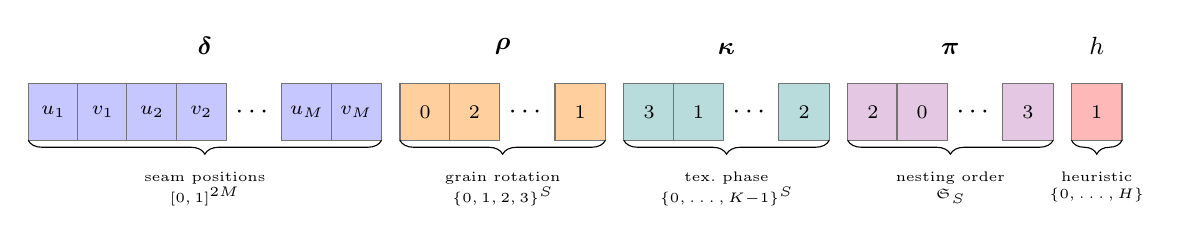
\begin{tikzpicture}[
  % ---- styles ----
  cell/.style 2 args={%
    draw=black!55, fill=#1, minimum width=#2, minimum height=0.72cm,
    inner sep=2pt, font=\scriptsize, align=center, outer sep=0pt,
  },
  dotcell/.style={%
    minimum width=0.52cm, minimum height=0.72cm, font=\normalsize,
    align=center, outer sep=0pt,
  },
  gaplabel/.style={minimum width=0.18cm, outer sep=0pt},
  brlabel/.style={font=\tiny, align=center},
]

% ---- colour palette ----
\colorlet{Cd}{blue!22}        % δ  – seam positions
\colorlet{Cr}{orange!38}      % ρ  – grain rotation
\colorlet{Ck}{teal!28}        % κ  – texture phase
\colorlet{Cp}{violet!22}      % π  – nesting order
\colorlet{Ch}{red!28}         % h  – heuristic

\def\cw{0.64cm}   % standard cell width
\def\sw{0.52cm}   % dots / spacer width

% =========================================================
% δ  –  u1 v1  u2 v2  ...  uM vM
% =========================================================
\node[cell={Cd}{\cw}]                        (d00) at (0,0)   {$u_1$};
\node[cell={Cd}{\cw}, right=-\pgflinewidth of d00] (d01)         {$v_1$};
\node[cell={Cd}{\cw}, right=-\pgflinewidth of d01] (d10)         {$u_2$};
\node[cell={Cd}{\cw}, right=-\pgflinewidth of d10] (d11)         {$v_2$};
\node[dotcell,         right=0pt             of d11] (ddots)      {$\cdots$};
\node[cell={Cd}{\cw}, right=0pt             of ddots] (dM0)       {$u_M$};
\node[cell={Cd}{\cw}, right=-\pgflinewidth  of dM0] (dM1)         {$v_M$};

% gap between δ and ρ
\node[gaplabel, right=0pt of dM1] (gap1) {};

% =========================================================
% ρ  –  ρ1 ρ2 ... ρS
% =========================================================
\node[cell={Cr}{\cw}, right=0pt of gap1]     (r1)  {$0$};
\node[cell={Cr}{\cw}, right=-\pgflinewidth of r1] (r2) {$2$};
\node[dotcell,         right=0pt of r2]      (rdots) {$\cdots$};
\node[cell={Cr}{\cw}, right=0pt of rdots]    (rS)  {$1$};

\node[gaplabel, right=0pt of rS] (gap2) {};

% =========================================================
% κ  –  κ1 κ2 ... κS
% =========================================================
\node[cell={Ck}{\cw}, right=0pt of gap2]     (k1)  {$3$};
\node[cell={Ck}{\cw}, right=-\pgflinewidth of k1] (k2) {$1$};
\node[dotcell,         right=0pt of k2]      (kdots) {$\cdots$};
\node[cell={Ck}{\cw}, right=0pt of kdots]    (kS)  {$2$};

\node[gaplabel, right=0pt of kS] (gap3) {};

% =========================================================
% π  –  π1 π2 ... πS
% =========================================================
\node[cell={Cp}{\cw}, right=0pt of gap3]     (p1)  {$2$};
\node[cell={Cp}{\cw}, right=-\pgflinewidth of p1] (p2) {$0$};
\node[dotcell,         right=0pt of p2]      (pdots) {$\cdots$};
\node[cell={Cp}{\cw}, right=0pt of pdots]    (pS)  {$3$};

\node[gaplabel, right=0pt of pS] (gap4) {};

% =========================================================
% h  –  single cell
% =========================================================
\node[cell={Ch}{\cw}, right=0pt of gap4]     (h)   {$1$};

% =========================================================
% Section labels  (above each group)
% =========================================================
\node[font=\small\bfseries, above=0.25cm of $(d00.north)!0.5!(dM1.north)$]
    (Ld) {$\boldsymbol{\delta}$};
\node[font=\small\bfseries, above=0.25cm of $(r1.north)!0.5!(rS.north)$]
    (Lr) {$\boldsymbol{\rho}$};
\node[font=\small\bfseries, above=0.25cm of $(k1.north)!0.5!(kS.north)$]
    (Lk) {$\boldsymbol{\kappa}$};
\node[font=\small\bfseries, above=0.25cm of $(p1.north)!0.5!(pS.north)$]
    (Lp) {$\boldsymbol{\pi}$};
\node[font=\small\bfseries, above=0.25cm of h.north]
    (Lh) {$h$};

% =========================================================
% Braces + domain annotations  (below each group)
% =========================================================
\draw[decorate, decoration={brace, mirror, amplitude=5pt}]
    (d00.south west) -- (dM1.south east)
    node[brlabel, midway, below=8pt]
        {seam positions \\ $[0,1]^{2M}$};

\draw[decorate, decoration={brace, mirror, amplitude=5pt}]
    (r1.south west) -- (rS.south east)
    node[brlabel, midway, below=8pt]
        {grain rotation \\ $\{0,1,2,3\}^{S}$};

\draw[decorate, decoration={brace, mirror, amplitude=5pt}]
    (k1.south west) -- (kS.south east)
    node[brlabel, midway, below=8pt]
        {tex.\ phase \\ $\{0,\ldots,K{-}1\}^{S}$};

\draw[decorate, decoration={brace, mirror, amplitude=5pt}]
    (p1.south west) -- (pS.south east)
    node[brlabel, midway, below=8pt]
        {nesting order \\ $\mathfrak{S}_S$};

\draw[decorate, decoration={brace, mirror, amplitude=5pt}]
    (h.south west) -- (h.south east)
    node[brlabel, midway, below=8pt]
        {heuristic \\ $\{0,\ldots,H\}$};

% =========================================================
% Subscript index labels on δ cells  (optional — comment out if too busy)
% =========================================================
%\node[font=\tiny, below=1pt of d00.south] {$u_1$};
%\node[font=\tiny, below=1pt of d01.south] {$v_1$};

\end{tikzpicture}
\end{document}
   (inside a figure environment)
%
% Layout:
%   δ (seam positions, continuous)  |  ρ (grain rotation)  |  κ (tex. phase)  |  π (nesting order)  |  h
%   2M floats in [0,1]              |  S ints in {0..3}    |  S ints in {0..K-1}  |  S-permutation  |  int

\documentclass[tikz, border=6pt]{standalone}
\usepackage{tikz}
\usetikzlibrary{decorations.pathreplacing, calc, positioning}
\usepackage{amsmath}
\usepackage{amssymb}

\begin{document}
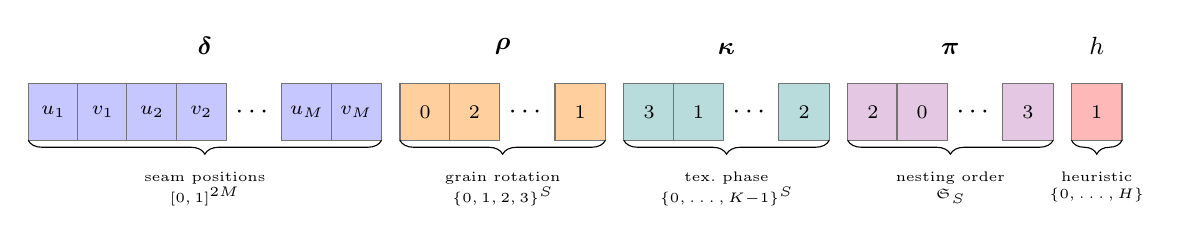
\begin{tikzpicture}[
  % ---- styles ----
  cell/.style 2 args={%
    draw=black!55, fill=#1, minimum width=#2, minimum height=0.72cm,
    inner sep=2pt, font=\scriptsize, align=center, outer sep=0pt,
  },
  dotcell/.style={%
    minimum width=0.52cm, minimum height=0.72cm, font=\normalsize,
    align=center, outer sep=0pt,
  },
  gaplabel/.style={minimum width=0.18cm, outer sep=0pt},
  brlabel/.style={font=\tiny, align=center},
]

% ---- colour palette ----
\colorlet{Cd}{blue!22}        % δ  – seam positions
\colorlet{Cr}{orange!38}      % ρ  – grain rotation
\colorlet{Ck}{teal!28}        % κ  – texture phase
\colorlet{Cp}{violet!22}      % π  – nesting order
\colorlet{Ch}{red!28}         % h  – heuristic

\def\cw{0.64cm}   % standard cell width
\def\sw{0.52cm}   % dots / spacer width

% =========================================================
% δ  –  u1 v1  u2 v2  ...  uM vM
% =========================================================
\node[cell={Cd}{\cw}]                        (d00) at (0,0)   {$u_1$};
\node[cell={Cd}{\cw}, right=-\pgflinewidth of d00] (d01)         {$v_1$};
\node[cell={Cd}{\cw}, right=-\pgflinewidth of d01] (d10)         {$u_2$};
\node[cell={Cd}{\cw}, right=-\pgflinewidth of d10] (d11)         {$v_2$};
\node[dotcell,         right=0pt             of d11] (ddots)      {$\cdots$};
\node[cell={Cd}{\cw}, right=0pt             of ddots] (dM0)       {$u_M$};
\node[cell={Cd}{\cw}, right=-\pgflinewidth  of dM0] (dM1)         {$v_M$};

% gap between δ and ρ
\node[gaplabel, right=0pt of dM1] (gap1) {};

% =========================================================
% ρ  –  ρ1 ρ2 ... ρS
% =========================================================
\node[cell={Cr}{\cw}, right=0pt of gap1]     (r1)  {$0$};
\node[cell={Cr}{\cw}, right=-\pgflinewidth of r1] (r2) {$2$};
\node[dotcell,         right=0pt of r2]      (rdots) {$\cdots$};
\node[cell={Cr}{\cw}, right=0pt of rdots]    (rS)  {$1$};

\node[gaplabel, right=0pt of rS] (gap2) {};

% =========================================================
% κ  –  κ1 κ2 ... κS
% =========================================================
\node[cell={Ck}{\cw}, right=0pt of gap2]     (k1)  {$3$};
\node[cell={Ck}{\cw}, right=-\pgflinewidth of k1] (k2) {$1$};
\node[dotcell,         right=0pt of k2]      (kdots) {$\cdots$};
\node[cell={Ck}{\cw}, right=0pt of kdots]    (kS)  {$2$};

\node[gaplabel, right=0pt of kS] (gap3) {};

% =========================================================
% π  –  π1 π2 ... πS
% =========================================================
\node[cell={Cp}{\cw}, right=0pt of gap3]     (p1)  {$2$};
\node[cell={Cp}{\cw}, right=-\pgflinewidth of p1] (p2) {$0$};
\node[dotcell,         right=0pt of p2]      (pdots) {$\cdots$};
\node[cell={Cp}{\cw}, right=0pt of pdots]    (pS)  {$3$};

\node[gaplabel, right=0pt of pS] (gap4) {};

% =========================================================
% h  –  single cell
% =========================================================
\node[cell={Ch}{\cw}, right=0pt of gap4]     (h)   {$1$};

% =========================================================
% Section labels  (above each group)
% =========================================================
\node[font=\small\bfseries, above=0.25cm of $(d00.north)!0.5!(dM1.north)$]
    (Ld) {$\boldsymbol{\delta}$};
\node[font=\small\bfseries, above=0.25cm of $(r1.north)!0.5!(rS.north)$]
    (Lr) {$\boldsymbol{\rho}$};
\node[font=\small\bfseries, above=0.25cm of $(k1.north)!0.5!(kS.north)$]
    (Lk) {$\boldsymbol{\kappa}$};
\node[font=\small\bfseries, above=0.25cm of $(p1.north)!0.5!(pS.north)$]
    (Lp) {$\boldsymbol{\pi}$};
\node[font=\small\bfseries, above=0.25cm of h.north]
    (Lh) {$h$};

% =========================================================
% Braces + domain annotations  (below each group)
% =========================================================
\draw[decorate, decoration={brace, mirror, amplitude=5pt}]
    (d00.south west) -- (dM1.south east)
    node[brlabel, midway, below=8pt]
        {seam positions \\ $[0,1]^{2M}$};

\draw[decorate, decoration={brace, mirror, amplitude=5pt}]
    (r1.south west) -- (rS.south east)
    node[brlabel, midway, below=8pt]
        {grain rotation \\ $\{0,1,2,3\}^{S}$};

\draw[decorate, decoration={brace, mirror, amplitude=5pt}]
    (k1.south west) -- (kS.south east)
    node[brlabel, midway, below=8pt]
        {tex.\ phase \\ $\{0,\ldots,K{-}1\}^{S}$};

\draw[decorate, decoration={brace, mirror, amplitude=5pt}]
    (p1.south west) -- (pS.south east)
    node[brlabel, midway, below=8pt]
        {nesting order \\ $\mathfrak{S}_S$};

\draw[decorate, decoration={brace, mirror, amplitude=5pt}]
    (h.south west) -- (h.south east)
    node[brlabel, midway, below=8pt]
        {heuristic \\ $\{0,\ldots,H\}$};

% =========================================================
% Subscript index labels on δ cells  (optional — comment out if too busy)
% =========================================================
%\node[font=\tiny, below=1pt of d00.south] {$u_1$};
%\node[font=\tiny, below=1pt of d01.south] {$v_1$};

\end{tikzpicture}
\end{document}
   (inside a figure environment)
%
% Layout:
%   δ (seam positions, continuous)  |  ρ (grain rotation)  |  κ (tex. phase)  |  π (nesting order)  |  h
%   2M floats in [0,1]              |  S ints in {0..3}    |  S ints in {0..K-1}  |  S-permutation  |  int

\documentclass[tikz, border=6pt]{standalone}
\usepackage{tikz}
\usetikzlibrary{decorations.pathreplacing, calc, positioning}
\usepackage{amsmath}
\usepackage{amssymb}

\begin{document}
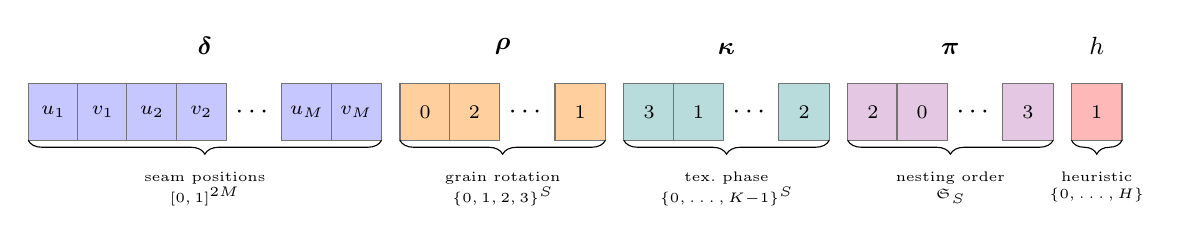
\begin{tikzpicture}[
  % ---- styles ----
  cell/.style 2 args={%
    draw=black!55, fill=#1, minimum width=#2, minimum height=0.72cm,
    inner sep=2pt, font=\scriptsize, align=center, outer sep=0pt,
  },
  dotcell/.style={%
    minimum width=0.52cm, minimum height=0.72cm, font=\normalsize,
    align=center, outer sep=0pt,
  },
  gaplabel/.style={minimum width=0.18cm, outer sep=0pt},
  brlabel/.style={font=\tiny, align=center},
]

% ---- colour palette ----
\colorlet{Cd}{blue!22}        % δ  – seam positions
\colorlet{Cr}{orange!38}      % ρ  – grain rotation
\colorlet{Ck}{teal!28}        % κ  – texture phase
\colorlet{Cp}{violet!22}      % π  – nesting order
\colorlet{Ch}{red!28}         % h  – heuristic

\def\cw{0.64cm}   % standard cell width
\def\sw{0.52cm}   % dots / spacer width

% =========================================================
% δ  –  u1 v1  u2 v2  ...  uM vM
% =========================================================
\node[cell={Cd}{\cw}]                        (d00) at (0,0)   {$u_1$};
\node[cell={Cd}{\cw}, right=-\pgflinewidth of d00] (d01)         {$v_1$};
\node[cell={Cd}{\cw}, right=-\pgflinewidth of d01] (d10)         {$u_2$};
\node[cell={Cd}{\cw}, right=-\pgflinewidth of d10] (d11)         {$v_2$};
\node[dotcell,         right=0pt             of d11] (ddots)      {$\cdots$};
\node[cell={Cd}{\cw}, right=0pt             of ddots] (dM0)       {$u_M$};
\node[cell={Cd}{\cw}, right=-\pgflinewidth  of dM0] (dM1)         {$v_M$};

% gap between δ and ρ
\node[gaplabel, right=0pt of dM1] (gap1) {};

% =========================================================
% ρ  –  ρ1 ρ2 ... ρS
% =========================================================
\node[cell={Cr}{\cw}, right=0pt of gap1]     (r1)  {$0$};
\node[cell={Cr}{\cw}, right=-\pgflinewidth of r1] (r2) {$2$};
\node[dotcell,         right=0pt of r2]      (rdots) {$\cdots$};
\node[cell={Cr}{\cw}, right=0pt of rdots]    (rS)  {$1$};

\node[gaplabel, right=0pt of rS] (gap2) {};

% =========================================================
% κ  –  κ1 κ2 ... κS
% =========================================================
\node[cell={Ck}{\cw}, right=0pt of gap2]     (k1)  {$3$};
\node[cell={Ck}{\cw}, right=-\pgflinewidth of k1] (k2) {$1$};
\node[dotcell,         right=0pt of k2]      (kdots) {$\cdots$};
\node[cell={Ck}{\cw}, right=0pt of kdots]    (kS)  {$2$};

\node[gaplabel, right=0pt of kS] (gap3) {};

% =========================================================
% π  –  π1 π2 ... πS
% =========================================================
\node[cell={Cp}{\cw}, right=0pt of gap3]     (p1)  {$2$};
\node[cell={Cp}{\cw}, right=-\pgflinewidth of p1] (p2) {$0$};
\node[dotcell,         right=0pt of p2]      (pdots) {$\cdots$};
\node[cell={Cp}{\cw}, right=0pt of pdots]    (pS)  {$3$};

\node[gaplabel, right=0pt of pS] (gap4) {};

% =========================================================
% h  –  single cell
% =========================================================
\node[cell={Ch}{\cw}, right=0pt of gap4]     (h)   {$1$};

% =========================================================
% Section labels  (above each group)
% =========================================================
\node[font=\small\bfseries, above=0.25cm of $(d00.north)!0.5!(dM1.north)$]
    (Ld) {$\boldsymbol{\delta}$};
\node[font=\small\bfseries, above=0.25cm of $(r1.north)!0.5!(rS.north)$]
    (Lr) {$\boldsymbol{\rho}$};
\node[font=\small\bfseries, above=0.25cm of $(k1.north)!0.5!(kS.north)$]
    (Lk) {$\boldsymbol{\kappa}$};
\node[font=\small\bfseries, above=0.25cm of $(p1.north)!0.5!(pS.north)$]
    (Lp) {$\boldsymbol{\pi}$};
\node[font=\small\bfseries, above=0.25cm of h.north]
    (Lh) {$h$};

% =========================================================
% Braces + domain annotations  (below each group)
% =========================================================
\draw[decorate, decoration={brace, mirror, amplitude=5pt}]
    (d00.south west) -- (dM1.south east)
    node[brlabel, midway, below=8pt]
        {seam positions \\ $[0,1]^{2M}$};

\draw[decorate, decoration={brace, mirror, amplitude=5pt}]
    (r1.south west) -- (rS.south east)
    node[brlabel, midway, below=8pt]
        {grain rotation \\ $\{0,1,2,3\}^{S}$};

\draw[decorate, decoration={brace, mirror, amplitude=5pt}]
    (k1.south west) -- (kS.south east)
    node[brlabel, midway, below=8pt]
        {tex.\ phase \\ $\{0,\ldots,K{-}1\}^{S}$};

\draw[decorate, decoration={brace, mirror, amplitude=5pt}]
    (p1.south west) -- (pS.south east)
    node[brlabel, midway, below=8pt]
        {nesting order \\ $\mathfrak{S}_S$};

\draw[decorate, decoration={brace, mirror, amplitude=5pt}]
    (h.south west) -- (h.south east)
    node[brlabel, midway, below=8pt]
        {heuristic \\ $\{0,\ldots,H\}$};

% =========================================================
% Subscript index labels on δ cells  (optional — comment out if too busy)
% =========================================================
%\node[font=\tiny, below=1pt of d00.south] {$u_1$};
%\node[font=\tiny, below=1pt of d01.south] {$v_1$};

\end{tikzpicture}
\end{document}
   (inside a figure environment)
%
% Layout:
%   δ (seam positions, continuous)  |  ρ (grain rotation)  |  κ (tex. phase)  |  π (nesting order)  |  h
%   2M floats in [0,1]              |  S ints in {0..3}    |  S ints in {0..K-1}  |  S-permutation  |  int

\documentclass[tikz, border=6pt]{standalone}
\usepackage{tikz}
\usetikzlibrary{decorations.pathreplacing, calc, positioning}
\usepackage{amsmath}
\usepackage{amssymb}

\begin{document}
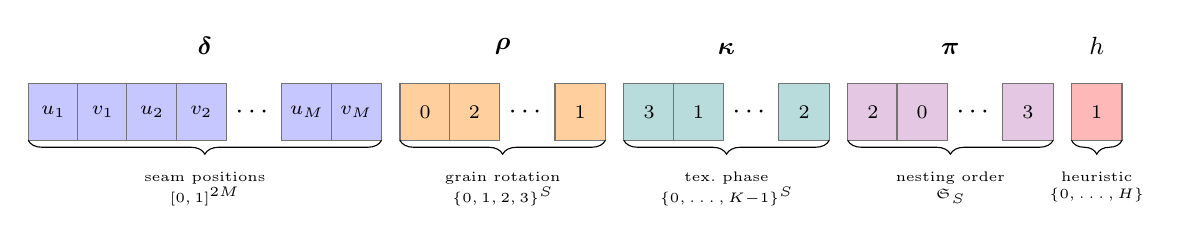
\begin{tikzpicture}[
  % ---- styles ----
  cell/.style 2 args={%
    draw=black!55, fill=#1, minimum width=#2, minimum height=0.72cm,
    inner sep=2pt, font=\scriptsize, align=center, outer sep=0pt,
  },
  dotcell/.style={%
    minimum width=0.52cm, minimum height=0.72cm, font=\normalsize,
    align=center, outer sep=0pt,
  },
  gaplabel/.style={minimum width=0.18cm, outer sep=0pt},
  brlabel/.style={font=\tiny, align=center},
]

% ---- colour palette ----
\colorlet{Cd}{blue!22}        % δ  – seam positions
\colorlet{Cr}{orange!38}      % ρ  – grain rotation
\colorlet{Ck}{teal!28}        % κ  – texture phase
\colorlet{Cp}{violet!22}      % π  – nesting order
\colorlet{Ch}{red!28}         % h  – heuristic

\def\cw{0.64cm}   % standard cell width
\def\sw{0.52cm}   % dots / spacer width

% =========================================================
% δ  –  u1 v1  u2 v2  ...  uM vM
% =========================================================
\node[cell={Cd}{\cw}]                        (d00) at (0,0)   {$u_1$};
\node[cell={Cd}{\cw}, right=-\pgflinewidth of d00] (d01)         {$v_1$};
\node[cell={Cd}{\cw}, right=-\pgflinewidth of d01] (d10)         {$u_2$};
\node[cell={Cd}{\cw}, right=-\pgflinewidth of d10] (d11)         {$v_2$};
\node[dotcell,         right=0pt             of d11] (ddots)      {$\cdots$};
\node[cell={Cd}{\cw}, right=0pt             of ddots] (dM0)       {$u_M$};
\node[cell={Cd}{\cw}, right=-\pgflinewidth  of dM0] (dM1)         {$v_M$};

% gap between δ and ρ
\node[gaplabel, right=0pt of dM1] (gap1) {};

% =========================================================
% ρ  –  ρ1 ρ2 ... ρS
% =========================================================
\node[cell={Cr}{\cw}, right=0pt of gap1]     (r1)  {$0$};
\node[cell={Cr}{\cw}, right=-\pgflinewidth of r1] (r2) {$2$};
\node[dotcell,         right=0pt of r2]      (rdots) {$\cdots$};
\node[cell={Cr}{\cw}, right=0pt of rdots]    (rS)  {$1$};

\node[gaplabel, right=0pt of rS] (gap2) {};

% =========================================================
% κ  –  κ1 κ2 ... κS
% =========================================================
\node[cell={Ck}{\cw}, right=0pt of gap2]     (k1)  {$3$};
\node[cell={Ck}{\cw}, right=-\pgflinewidth of k1] (k2) {$1$};
\node[dotcell,         right=0pt of k2]      (kdots) {$\cdots$};
\node[cell={Ck}{\cw}, right=0pt of kdots]    (kS)  {$2$};

\node[gaplabel, right=0pt of kS] (gap3) {};

% =========================================================
% π  –  π1 π2 ... πS
% =========================================================
\node[cell={Cp}{\cw}, right=0pt of gap3]     (p1)  {$2$};
\node[cell={Cp}{\cw}, right=-\pgflinewidth of p1] (p2) {$0$};
\node[dotcell,         right=0pt of p2]      (pdots) {$\cdots$};
\node[cell={Cp}{\cw}, right=0pt of pdots]    (pS)  {$3$};

\node[gaplabel, right=0pt of pS] (gap4) {};

% =========================================================
% h  –  single cell
% =========================================================
\node[cell={Ch}{\cw}, right=0pt of gap4]     (h)   {$1$};

% =========================================================
% Section labels  (above each group)
% =========================================================
\node[font=\small\bfseries, above=0.25cm of $(d00.north)!0.5!(dM1.north)$]
    (Ld) {$\boldsymbol{\delta}$};
\node[font=\small\bfseries, above=0.25cm of $(r1.north)!0.5!(rS.north)$]
    (Lr) {$\boldsymbol{\rho}$};
\node[font=\small\bfseries, above=0.25cm of $(k1.north)!0.5!(kS.north)$]
    (Lk) {$\boldsymbol{\kappa}$};
\node[font=\small\bfseries, above=0.25cm of $(p1.north)!0.5!(pS.north)$]
    (Lp) {$\boldsymbol{\pi}$};
\node[font=\small\bfseries, above=0.25cm of h.north]
    (Lh) {$h$};

% =========================================================
% Braces + domain annotations  (below each group)
% =========================================================
\draw[decorate, decoration={brace, mirror, amplitude=5pt}]
    (d00.south west) -- (dM1.south east)
    node[brlabel, midway, below=8pt]
        {seam positions \\ $[0,1]^{2M}$};

\draw[decorate, decoration={brace, mirror, amplitude=5pt}]
    (r1.south west) -- (rS.south east)
    node[brlabel, midway, below=8pt]
        {grain rotation \\ $\{0,1,2,3\}^{S}$};

\draw[decorate, decoration={brace, mirror, amplitude=5pt}]
    (k1.south west) -- (kS.south east)
    node[brlabel, midway, below=8pt]
        {tex.\ phase \\ $\{0,\ldots,K{-}1\}^{S}$};

\draw[decorate, decoration={brace, mirror, amplitude=5pt}]
    (p1.south west) -- (pS.south east)
    node[brlabel, midway, below=8pt]
        {nesting order \\ $\mathfrak{S}_S$};

\draw[decorate, decoration={brace, mirror, amplitude=5pt}]
    (h.south west) -- (h.south east)
    node[brlabel, midway, below=8pt]
        {heuristic \\ $\{0,\ldots,H\}$};

% =========================================================
% Subscript index labels on δ cells  (optional — comment out if too busy)
% =========================================================
%\node[font=\tiny, below=1pt of d00.south] {$u_1$};
%\node[font=\tiny, below=1pt of d01.south] {$v_1$};

\end{tikzpicture}
\end{document}
